\documentclass{article}
\usepackage{amsmath}
\usepackage{graphicx}
\usepackage{float}
\begin{document}
\section{Overview}
The largest and bulkiest device on any electrical vehicle is the battery.
Dense energy storage is a difficult task, and batteries are a must for almost all devices.
\section{Capacity}
The larger the capacity of a battery network, the larger, heavier, and more expensive the battery network becomes.
The use case of the system needs to be considered for choosing a capacity.
Capacitance is normally measured in Amp-Hours, or how many hours a battery can supply the rated current at the nominal voltage of the battery.

When specifying capacity for an electric vehicle, two factors are going to be needed:
\begin{itemize}
    \item Range
    \item Efficiency
\end{itemize}
The nominal range will be determined by the expected average daily usage, and the specified charge frequency. 
The value given for charge frequency will be once a week.
The daily usage will be a round trip from Josephine butler to the engineering department on the science site each way this is ~1.5km, this is shown in Fig. \ref{fig:route}.
\begin{figure}[H]
    \centering
    \scalebox{0.5}{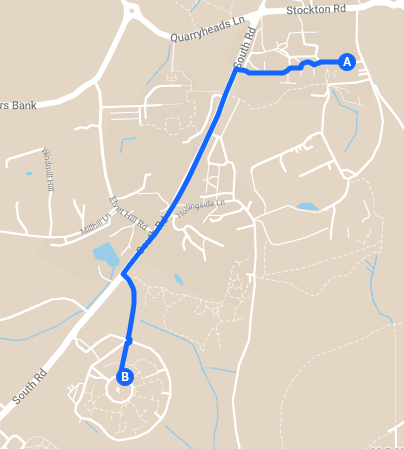
\includegraphics{./RouteAnalysis/Route.png}}
    \caption{Nominal daily route}
    \label{fig:route}
\end{figure}
The exact elevation change can be seen in \ref{fig:route_el}, with the gradients of this data in \ref{fig:route_grad}.
This data is taken from GPS public databases via https://www.gpsvisualizer.com/elevation.
The routes were made using google maps - exported to GPS route format.
\begin{figure}[H]
    \centering
    \scalebox{0.5}{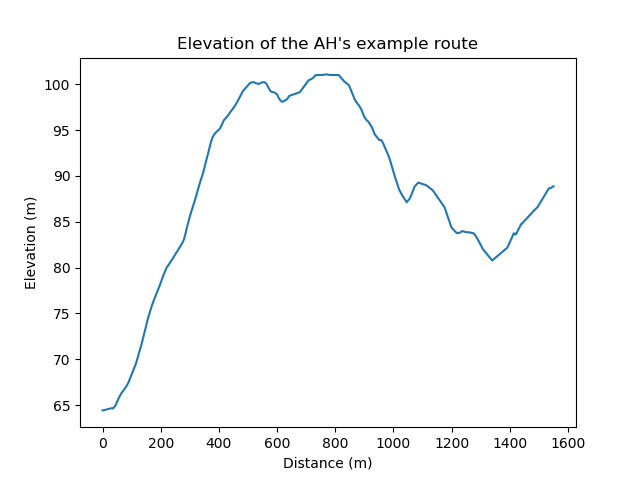
\includegraphics{./RouteAnalysis/elevation.png}}
    \caption{Gradient of route}
    \label{fig:route_el}
\end{figure}
Fig. \ref{fig:route_el} shows the elevation through the route, with mountjoy easily identifiable. 
\begin{figure}[H]
    \centering
    \scalebox{0.5}{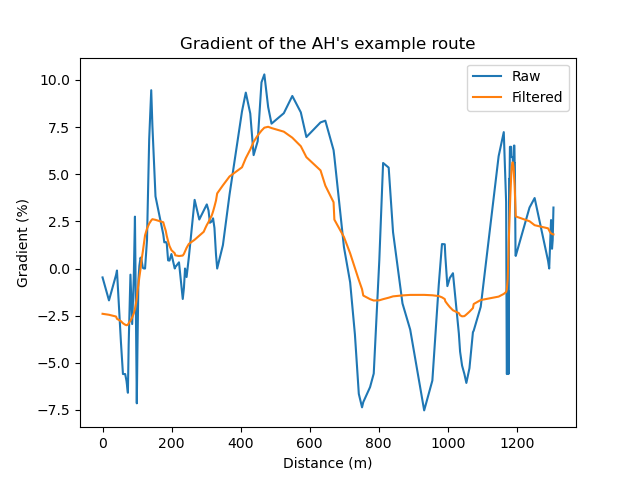
\includegraphics{./RouteAnalysis/grad.png}}
    \caption{Elevation of route}
    \label{fig:route_grad}
\end{figure}
There is a total of 50 meters uphill, and 25 meters downhill when going towards butler.
The effect of the height change on the required battery capacity will be non negligible.
If we model the energy requirement as a simple vehicle hoist, the energy will be $mg\Delta h$.
The total vertical distance is 75m.
Roughly 90kJ more energy will be needed with a perfectly efficient system.
Since a joule is one watt second, 60kJ is 25 watt hours.



Rough power estimates: 
10 watt hours per mile - electric bike
12 watt hours per journey (flat)

\section{Charging}
Battery charging is difficult, specific charging circuits are needed for most modern high density batteries.
When trying to charge lots of batteries quickly a large amount of heat is generated, which needs to be considered in the design stage.
Large modern batteries can also be very dangerous - and this is amplified when charging, so care needs to be taken that the design isn't a health hazard.
\subsection{Lifespan}
The lifespan of a battery is determined by the depth of discharge, and the family of battery used.
Lithium ion batteries have a cycle life of about 300 at a depth of discharge of 100\%, and a cycle life of about 800 cycles at 50\% DoD.
Lithium polymer batteries have a similar lifespan at 100\% DoD, but can increase up to 2000 charges at 50\% DoD.

For this reason we are using LiPo batteiers as they offer the best battery life-span in terms of cycle count.
\subsection{Rate of charge}
The rate of charging is a nonlinear funciton with the charge of the battery, therefore it doesn't to quote charge time from 0\%-100\%.
It makes sense to specify a rate of recharge from a specific depth of discharge.
The spesific depth of discharge will be determined by the lifespan of the battery, and we can consider a "charge cycle" charging from DoD\% to 95\%.

%https://www.dnkpower.com/lithium-polymer-battery-guide/
%https://batteryuniversity.com/learn/article/how_to_prolong_lithium_based_batteries
\section{Regenerative breaking}
Regenerative breaking is the process of turning unwanted mechanical energy (movement) into electrical energy that can charge the battery. 
This makes stop start traffic much more efficient - and large amounts of energy can be re-claimed by going downhill.
\end{document}
